\documentclass[letterpaper]{article}
\usepackage[letterpaper, left=0.625in, right=0.625in, bottom=1in, top=0.75in]{geometry}
\usepackage{cmap}
\usepackage{multicol}
\usepackage{cite}
\usepackage{float}
\usepackage{graphicx}
\usepackage[T1]{fontenc}
\usepackage{lmodern}
\usepackage{amsmath}

\title{Internship Report}
\author{Nathan Boyer}

\begin{document}

\maketitle

\begin{abstract}

    It's possible to distribute the Internet to users via drones.
    However it is then necessary to place the drones according to the positions of the users.
    Moreover, the 5th Generation (5G) New Radio (NR) technology is designed to accommodate a wide range of applications and industries. The NGNM 5G White Paper \cite{5gwhitepaper} groups these vertical use cases into three categories:
    \begin{enumerate}
        \item enhanced Mobile Broadband (eMBB)
        \item massive Machine Type Communication (mMTC)
        \item Ultra-Reliable Low-latency Communication (URLLC).
    \end{enumerate}

    A partitioning of the physical network into several virtual networks looks to be the most suitable approach to provide a customized service to each application and to limit the operation expenses. This design is well known as \textit{network slicing}.
    Each drone must thus slice its bandwith between each of the 3 user classes.
    This whole problem (placement + bandwidth) can be defined as an optimization problem, but since it is very hard to solve efficiently, it is almost always addressed by AI.
    In my internship, I wanted to prove that viewing the problem as an optimization problem can still be useful, by building an hybrid solution involving on one hand AI and on the other optimization.
    I use it to achieve better results than approaches that use only AI, although at the cost of slightly larger (but still reasonable) computation times.
\end{abstract}


\tableofcontents


\section{Probleme presentation and literature analysis}

The concept of network slicing has been investigated for some time. With the purpose of providing multiple core networks over the same network infrastructure, DECOR and eDECOR \cite{decor} have been already used in legacy LTE networks. 
However, the slicing of Radio Access Network (RAN) was not considered in these works yet.
Since then, the 5G network slicing concept evolved, by providing a better modularization and flexibility of the network functions.
RAN slicing is now of great interest for the literature, given the ability to support resource isolation among different slices, providing a way to allocate radio resources to the connected User Equipments (UEs) based on the slices they belong to. 
Several RAN slicing approaches have been proposed in the past few years. 
Traditional strategies (\hspace{1sp}\cite{RANslicing1}, \cite{orion})  mainly deal with orthogonal resource allocation in time and/or frequency domain, such that the isolation between different services is guaranteed. Their aim in mainly oriented at allocating virtual Resource Blocks (vRBs) to UEs for intra-slice scheduling and to map the allocated vRBs to Physical Resource Blocks (PRBs) at a second stage.

Machine Learning (ML) techniques (\hspace{1sp}\cite{fairness}, \cite{main_article}), mainly deep reinforcement learning, have also been extensively considered, given their capability to find patterns within the huge amount of data that is exchanged in cellular networks.

In \textit{Deep Reinforcement Learning for Combined Coverage and Resource Allocation in UAV-Aided RAN-Slicing}\cite{main_article}, the authors develop a deep reinforcement learning agent that decides the best direction to go over a few 100 steps, and that is the most common approach.
Indeed, in \textit{UAV-Assisted Fair Communication for Mobile Networks: A Multi-Agent Deep Reinforcement Learning Approach}\cite{fairness}, the authors do pratically the same thing but add the dimension of fairness between the users.
Moreover, in \textit{QoS-Aware UAV-BS Deployment Optimization Based on Reinforcement Learning}\cite{deep-qn}, the authors show that using deep-Q-network, it is possible to achieve optimal performance when placing only 1 base station.
Finally, in \textit{Reinforcement Learning Aided UAV Base Station Location Optimization for Rate Maximization}\cite{rate_max}, the authors use again deep reinforcement learning to resolve the placement of 3 UAVs and find that it achieves around 70\% of the optimal performance, and that it is better that a k-means algorithm when the measure of imperfection is higher.

My internship aims at developping the following points on a 2-UAVs-aided RAN slicing:

\begin{enumerate}
    \item Improving the optimization algorithm to make it able to generate big amount of data in reasonable time
    \item Developping an AI agent that learns from the optimal optimization algorithm with supervised learning
    \item Building an hybrid agent from this AI agent that combines AI and algorithmic to achieve better performance
    \item Realizing an honest comparaison between the different methods both in terms of performance achieved and in terms of computation time
\end{enumerate}


\section{Problem solving by constrained optimization}

\subsection{In-depth explanation}

This problem can be solved by constrained optimization (\hspace{1sp}\cite{main_article}).

First, we have to define the equation that computes how well a user will reveive a base station's connection depending on where it is.

We have the following Equations for the drones's SINRs, which is a factor that represents how much data is effectively receiveed by the user, in relation to the data sent by the base station to the user:

$\operatorname{SINR}_{i, j}^t=\frac{p c \mu\left(y_j, u_i^t\right)\left(\left(\left\|y_j-u_i^t\right\|\right)^2+\left(h\right)^2\right)^{-\alpha / 2}}{\sum\limits_{k \in \mathcal{U} \backslash i} p c \mu\left(y_j, u_k^t\right)\left(\left(\left\|y_j-u_k^t\right\|\right)^2+\left(h\right)^2\right)^{-\alpha / 2}+\sigma^2}$

To evaluate a configuration we will thus proceed as follows:

You first need to associate each user with its nearest base station.

You then share the bandwidth of a base station dedicated to a given class between all users of this class associated to this base station.

Then, you compute each user SINR and decide for the user is satisfied or not.

The percentage of satisfied user is thus what you want to maximize.

\subsection{Optimization problem}

This problem can be resolved by as an optimization problem, I will show you how to resolve it for 2 base stations.

Let's first define u a matrix of dimensions $N*N$, with N being the number of positions possible for a base station.
$u_{i,j}$ is a binary variable that is equal to one if and only if the first base station is in position i and the second is position j.

$bw$ is a $3*2$ matrix that represents the bandwidth each base station allocates to each user class.

$\delta$ is a vector that represents for every whether it is satisfied or not.

The function to optimize is then: $\max_{u,bw}\sum_{g\in\mathcal{G}}\delta_g$

Under the following constraints:

\begin{subequations}
    \allowdisplaybreaks
    \begin{align}
        & \sum_{b \in |\mathcal{U}|} \sum_{i, j \in \mathcal{U}} u_{i, j} \times bw_{\text{slice}(g), b} \times \text{bps}_g \frac{100}{G_{\text{conn}}(\text{slice}(g),b)} \nonumber \\
        & \geq th_g \times \delta_g \hspace{1cm} \forall g \in \mathcal{G} \\[1em]
        & bw_{em,b} + bw_{ur,b} + bw_{mm,b} = 1 \hspace{1cm} \forall b \in |\mathcal{U}| \\[1em]
        & bw_{em,b} \geq 0; bw_{ur,b} \geq 0; bw_{mm,b} \geq 0 \hspace{1cm} \forall b \in |\mathcal{U}| \\[1em]
        & \sum_{i,j \in \mathcal{U}}u_{i,j} = 1 \\[1em]
        & \delta_g \in \{0, 1\} \hspace{1cm} \forall g \in \mathcal{G} \\[1em] 
        & u_{i,j} \in \{0, 1\} \hspace{1cm} \forall i,j \in \{0, 1, ... , |\mathcal{U}-1|\}
    \end{align}\label{constr}
    \end{subequations}

The resolution of this optimization problem can be implemented in Python with the help of a module such as pulp.

\subsection{Instances generation}

This internship is mainly based on this article: \textit{Deep Reinforcement Learning for Combined Coverage and Resource Allocation in UAV-Aided RAN-Slicing}\cite{main_article}.
As such, instances of the problem are generated in a very similar way as they are in this article, and are as follows:

\begin{table}[H]
    \centering
    \begin{tabular}{|c|c|}
    \hline
    Parameter & Value \\
    \hline
        Number of users $n$ & 50 (later 25 - 100)\\
        Number of clusters $c$ & 2 (later 0 - 5) \\
        UAV transmit power $p$ &  1 W\\
        pathloss exponend $\alpha$ & 2.1 \cite{Channel_Model}\\
        UAV half-power beamwidth $\eta$ & 30 deg. \cite{Channel_Model}\\
        Near-field pathloss $c$ & -38.4 dB \cite{Channel_Model}\\
        Noise power $\sigma^2$ & $8 \cdot 10^{-13}$ W\\
        Bandwidth $B$ & 20 MHz\\
        Users density, $|\mathcal{G}|/\text{km}^2$ & 100\\
        UAVs number, $|\mathcal{U}|$ & 2\\
        UAVs height $h$ & 50 m\\
        UAVs density $|\mathcal{U}|/\text{km}^2$ & 8\\
        eMBB users demand $\text{dem}_\text{eMBB}$ & 5 Mbps \cite{demandsvalues}\\
        URLLC users demand $\text{dem}_\text{URLLC}$ & 10 Mbps \cite{demandsvalues}\\
        mMTC users demand $\text{dem}_\text{mMTC}$ & 0.5 Mbps \cite{demandsvalues}\\
        $p_{\text{eMBB}}$, $p_{\text{URLLC}}$, $p_{\text{mMTC}}$ & 20\%, 10\%, 70\% \\
    \hline
    \end{tabular}
    \caption{Environment Parameters}
    \label{tab:envparams}
\end{table}


\subsection{Improvement of the optimization algorithm}

To speed up the resolution of this problem, I implemented a few optimizations:

First, only positions in the convex enveloppe of the users can actually be candidates for optimal placements of the base stations.
We can thus reduce by a lot the size of the matrix u.

Moreover, it is possible to go further but not without losing precision.
Indeed, you can divide the users into k clusters and take the union of this convex enveloppe of this clusters.

You can visualize the transformation done as follows:

\begin{figure}[H]
    \centering
    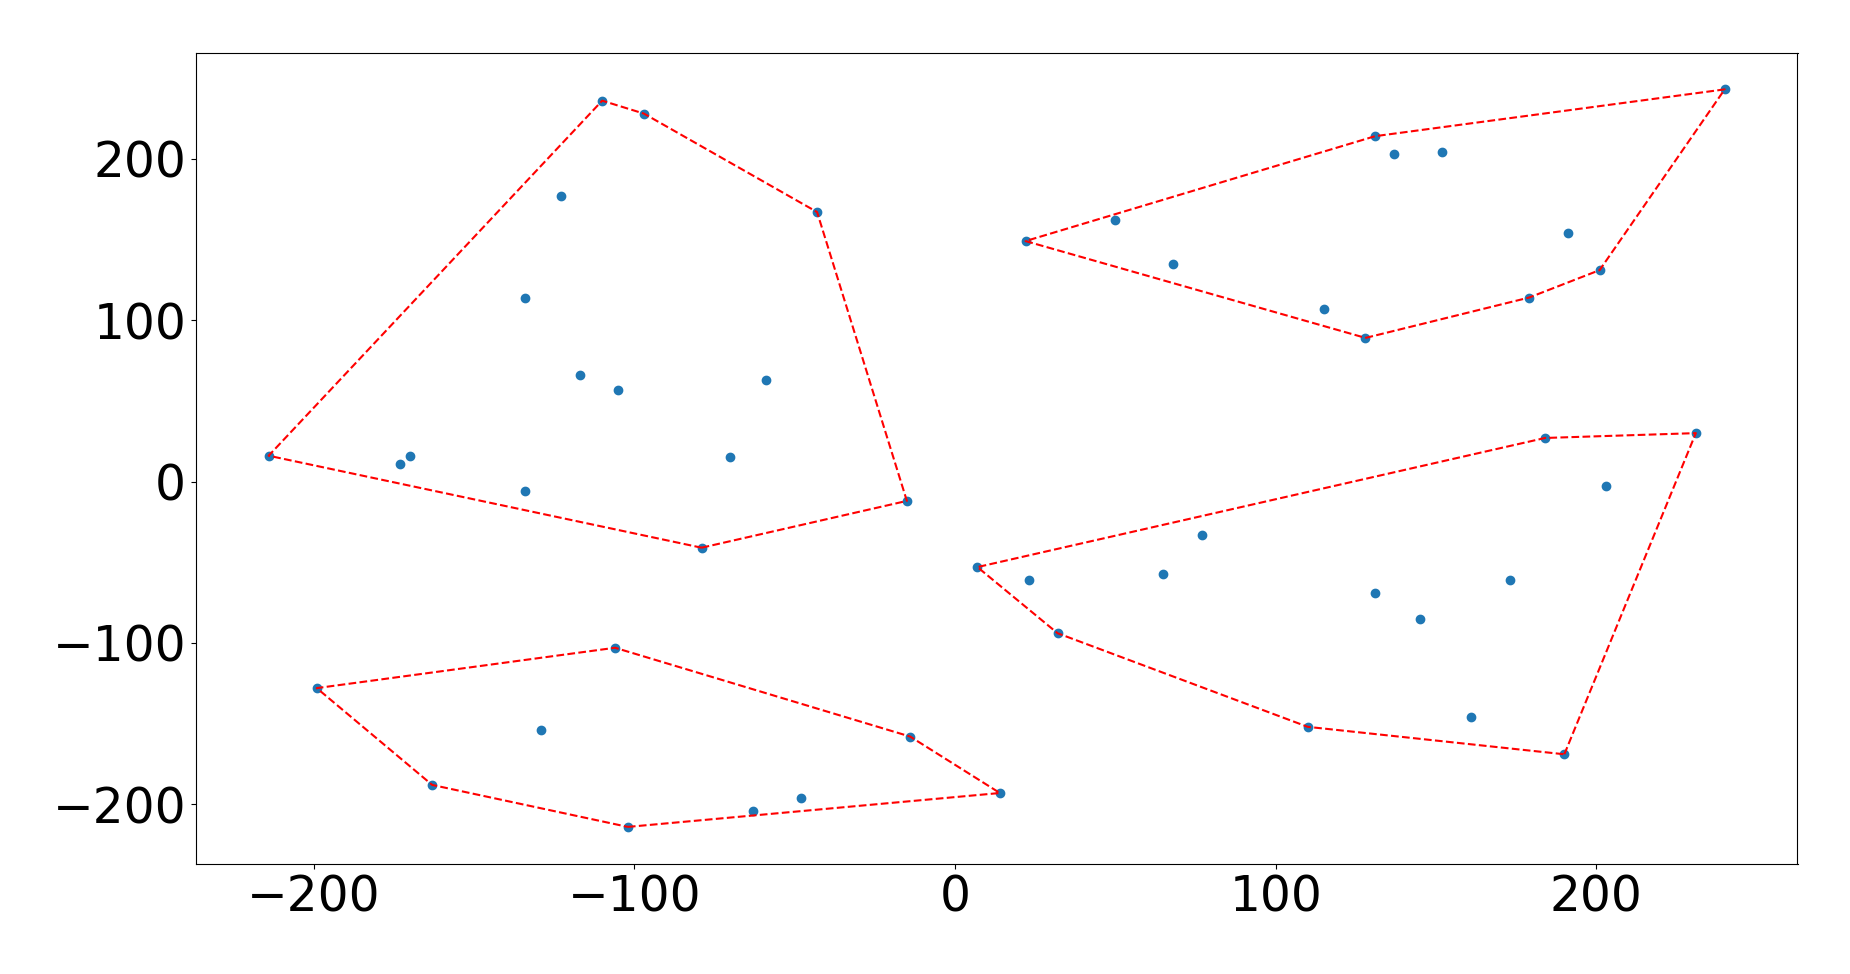
\includegraphics[width=0.5\textwidth]{images/four_cluster.png}
    \caption{Representation of the convex enveloppe of the 4 clusters}
\end{figure}

The graph of performance and time in function of the number of clusters can be found below.

Moreover, I am using \textit{Quote article here} to generate instances, thus as the instances generated have as many
clusters as they have base stations, I am going to generate instances using clusters too.
The performances are then as follows:

\begin{figure}[H]
    \centering
    \begin{minipage}[b]{0.45\textwidth}
        \centering
        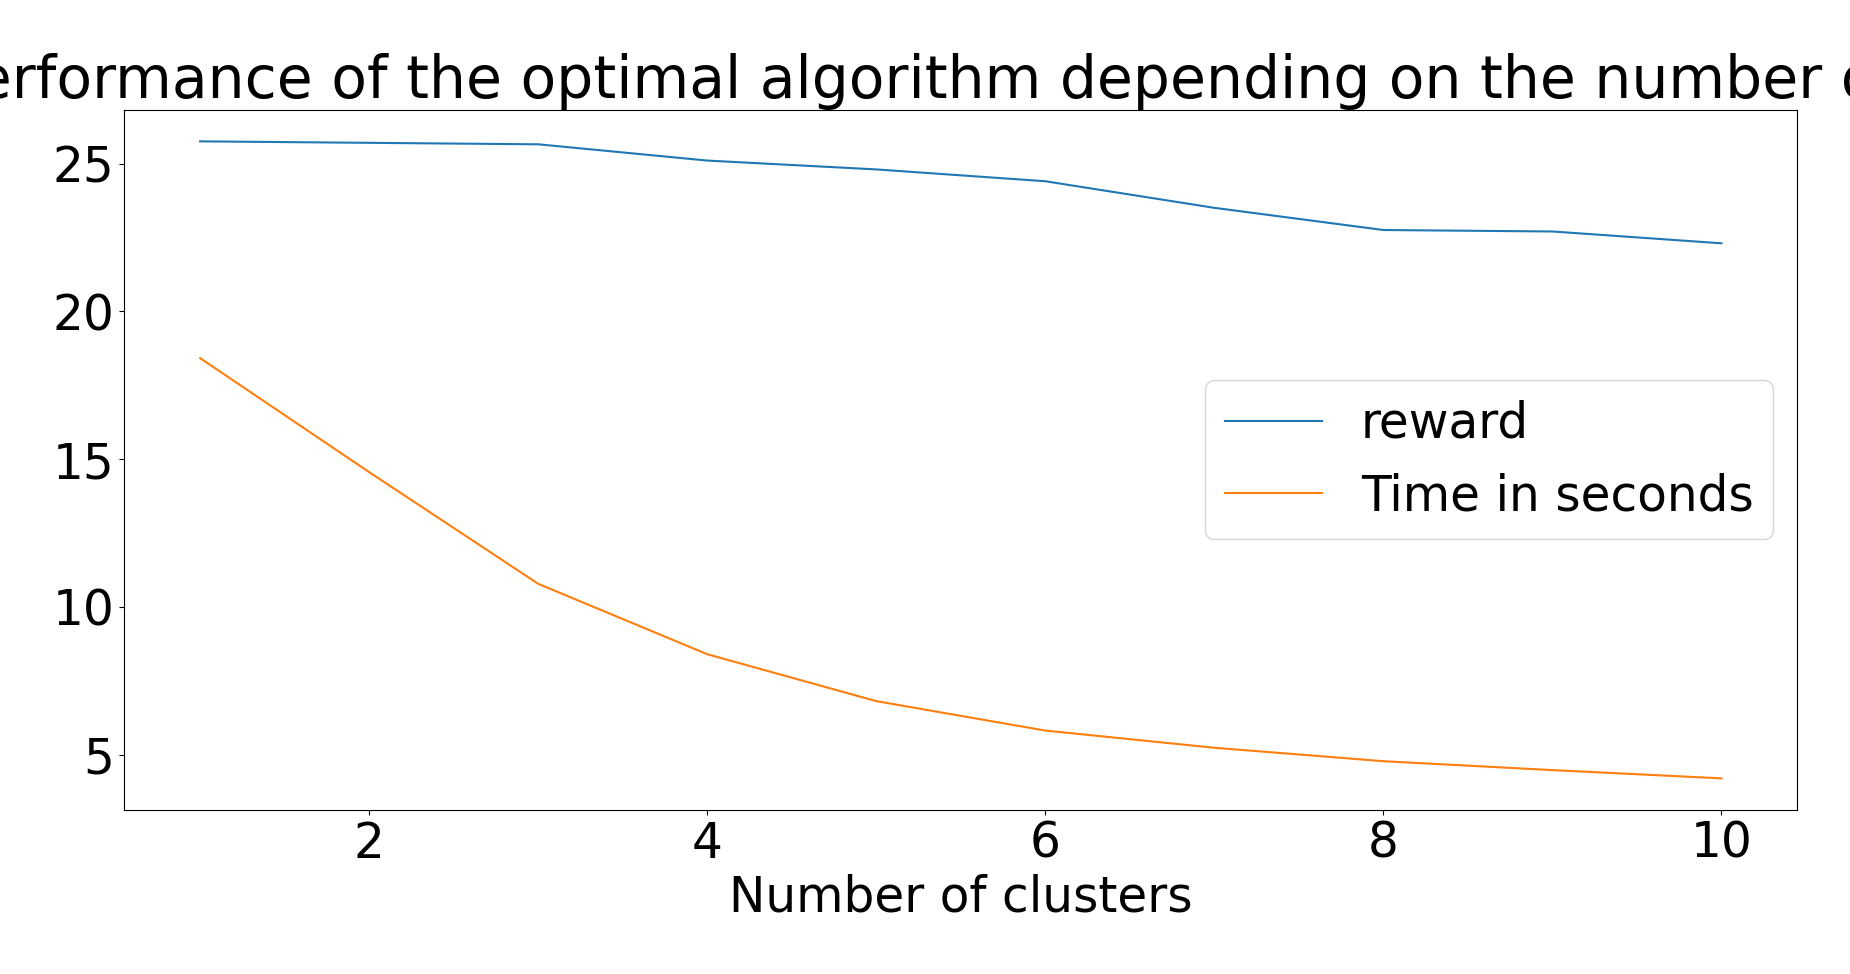
\includegraphics[width=\textwidth]{images/Performance_opt_function_clusters.png}
        \caption{Performance when users are random}
    \end{minipage}
    \hspace{0.05\textwidth}
    \begin{minipage}[b]{0.45\textwidth}
        \centering
        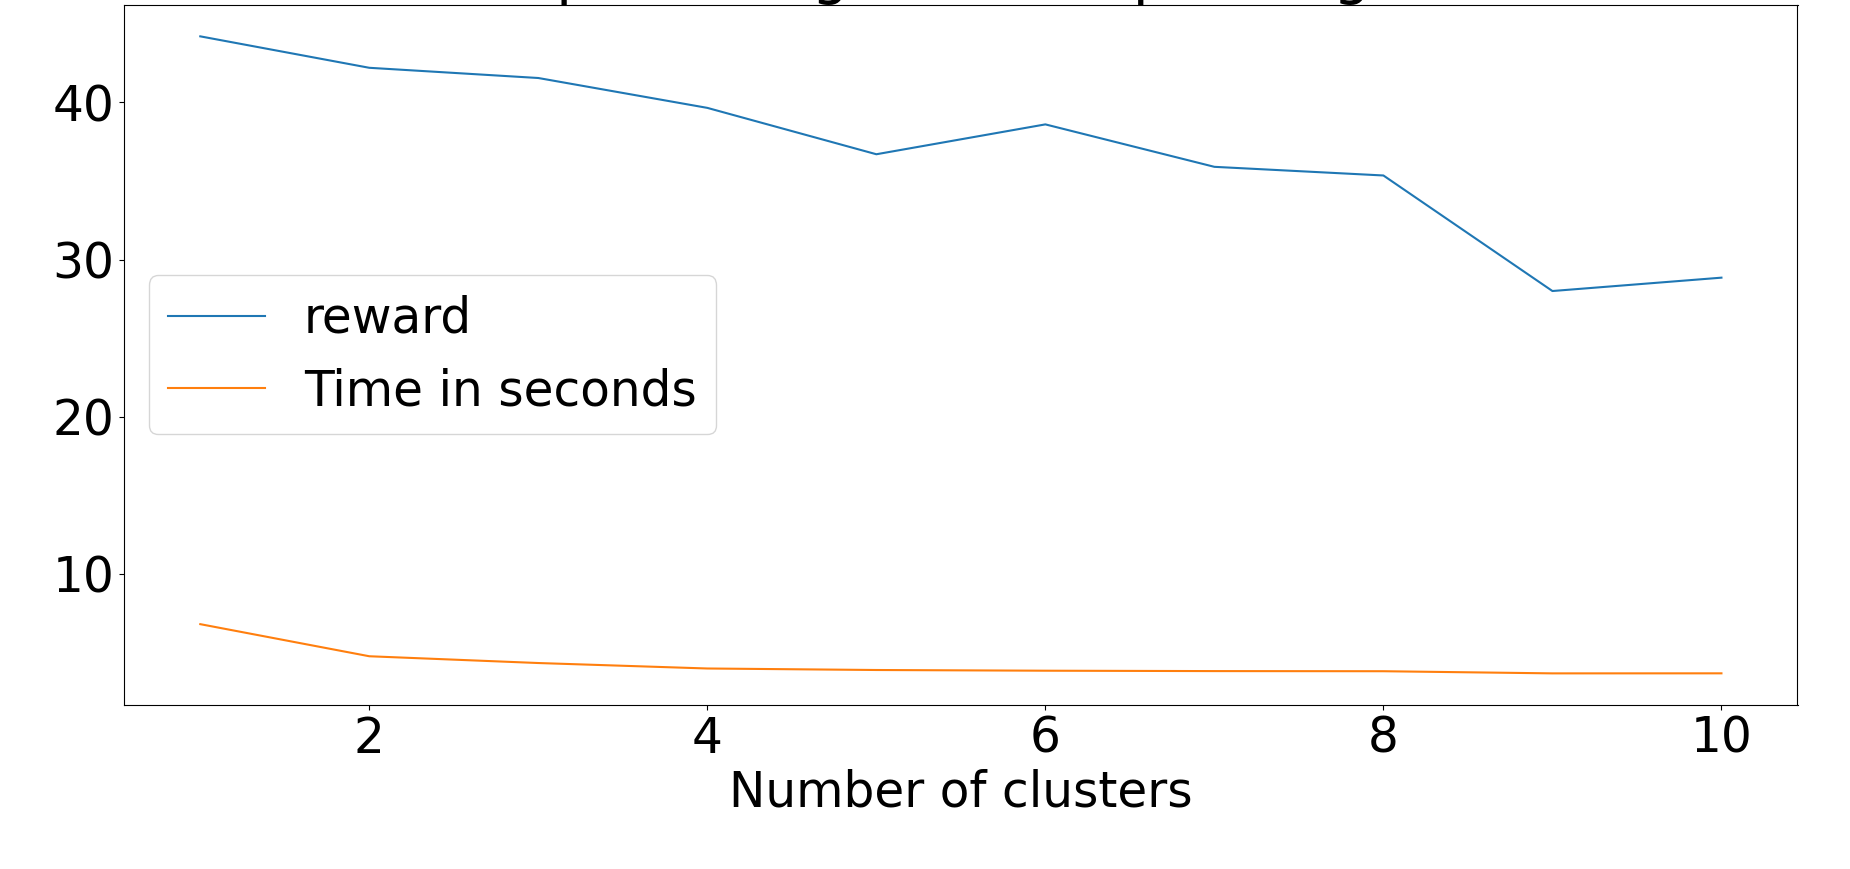
\includegraphics[width=\textwidth]{images/Performance_opt_function_clusters_when_2clusters.png}
        \caption{Performance when users are in 2 clusters}
    \end{minipage}
\end{figure}

However, since the computation times are pretty reasonable for 2 base stations, I decided to go with only 1 cluster.

Finally, multithreading can be used to further accelerate the computations.

\section{Machine learning to solve the problem}

However, a major issue is that this method of solving the problem by optimization is still pretty long.
This can be problematic, especially if the users are moving, and it thus becomes necessary to recalculate the optimal position often.

Thus, a solution using machine learning was considered.
Indeed, solving an instance of the problem would only require a forward pass of the neural network, which is negligible in time.

\subsection{Reinforcement learning}

A reinforcement learning solution was imagined and implemented, again in article\;\cite{main_article}

The authors tried to solve the same problem as the one I presented and, to put it shortly, managed to get an average reward of 72-73\% of users satisfied.

However, there are multiple differences between how they approached this problem and how I did:

\begin{enumerate}
    \item First, they move the base stations setp by step and computes the mean reward over 100 movements.
          However, since the base stations spend most of their times idling (because they have already reached their best possible position),
          I took the bias of putting the base stations directly at the computed best position, and then computing the reward only once (which also allows to test the different agents over more instances in the same amount of time).
    \item Secondly, what is plotted in their article is the average reward during the reinforcement process.
          What it means is that the neural network is only tested on the instances it just learnt from.
          What I did instead is I have a separate test set, which I use to evaluate the different agents.
\end{enumerate}

\subsection{Supervised learning from the optimal solution}

But, an other idea is to use supervised learning.
By using an optimal agent, the neural network can learn to replicate the optimal solutions.
Developping such an AI was the initial subject of my internship.

The neural network is thus divided in 2 neural networks:

\begin{enumerate}
    \item A neural network that takes as inputs the positions of the users and learns to output the best positions for the 2 base stations.
    \item A neural network that takes as inputs the positions of the users and the positions of the base stations and learns to output the best slicing of bandwiths between the 3 classes of users.
\end{enumerate}

As a side note, the type of each users is represented by 3 one-hots, one for each of the class.
More details about how the neural networks are built are avaible in the appendix

To conclude with my results, here is the average error for the neural network that learns to output the positions:
As well as the average error for the neural network that learns to output the bandwiths:

\begin{figure}[H]
    \centering
    \begin{minipage}[b]{0.45\textwidth}
        \centering
        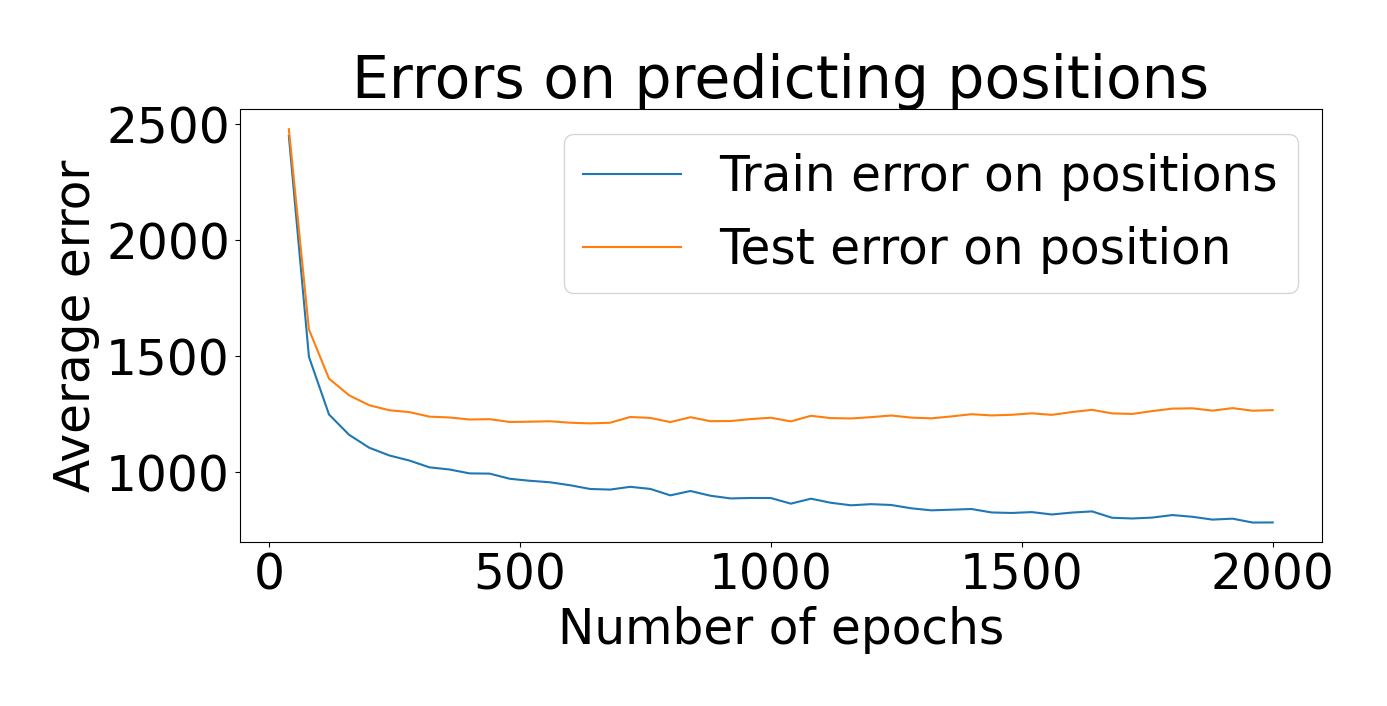
\includegraphics[width=\textwidth]{images/mix_pos.png}
        \caption{Position error}
        \label{fig:image5}
    \end{minipage}
    \hspace{0.05\textwidth}
    \begin{minipage}[b]{0.45\textwidth}
        \centering
        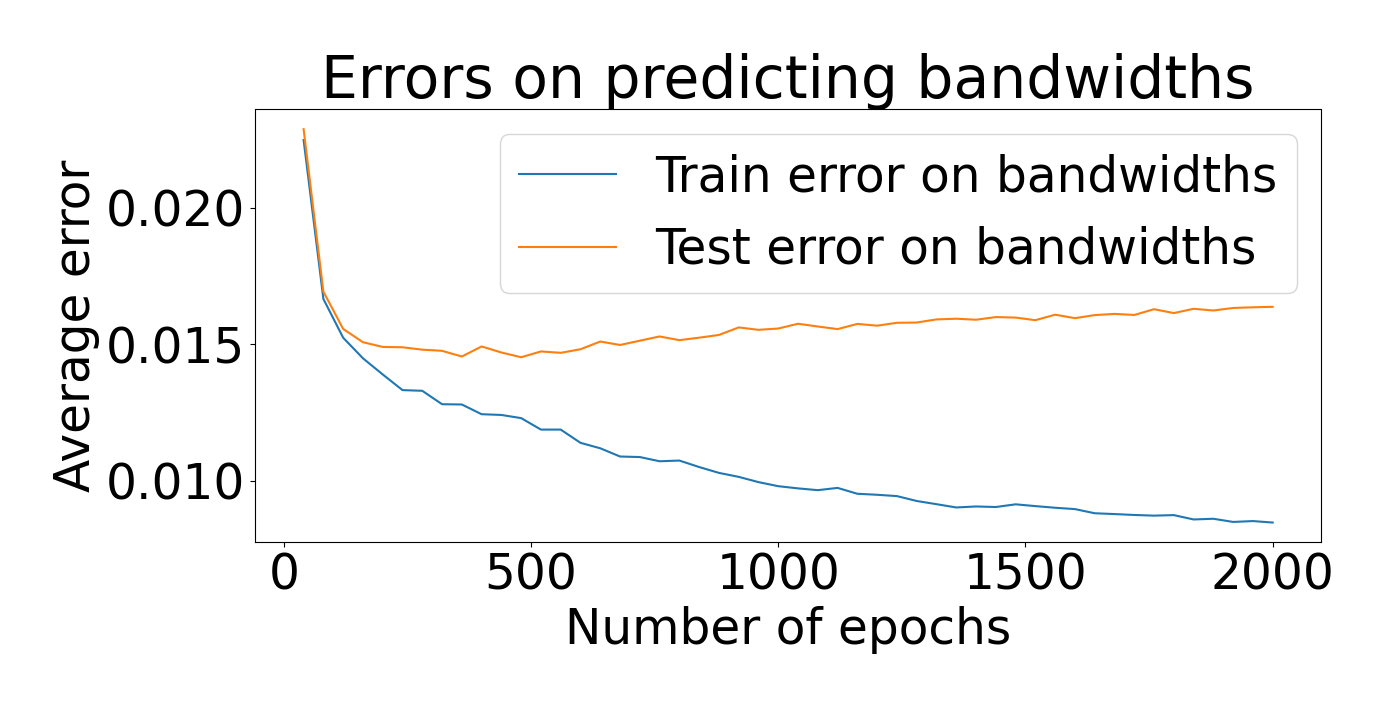
\includegraphics[width=\textwidth]{images/bw_error_epochs.png}
        \caption{Bandwidth error}
        \label{fig:image6}
    \end{minipage}
\end{figure}

\;

With these neural networks, we can test it on instances and evaluate the performances it gives.

(We plot here the normalized average user coverage, i.e.\, the average user coverage divided by the average user coverage of the optimal solution)


\begin{figure}[H]
    \centering
    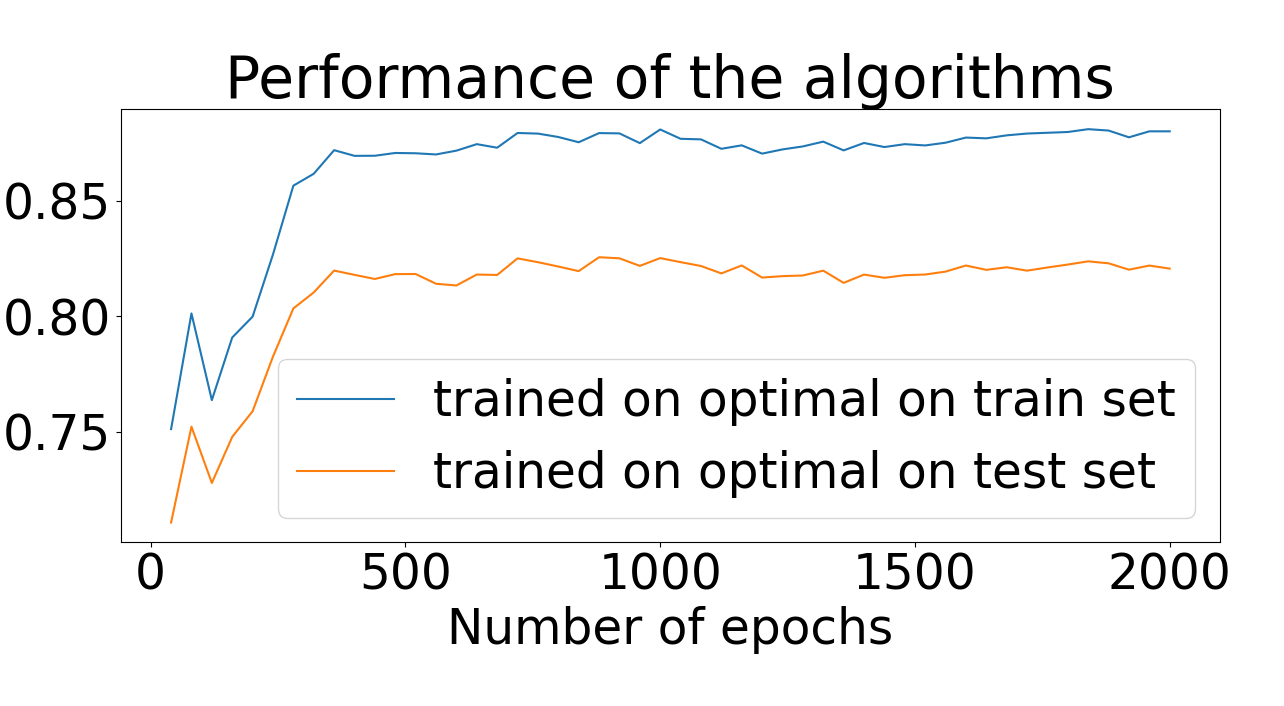
\includegraphics[width=0.5\textwidth]{images/bilan_en _fonction epochs.png}
    \caption{Normalized average user coverage for AI agent}
\end{figure}

\subsection{Learn only what's necessary}

However, you can see the test error on bandwiths stops to decrease rapidly.
That's why I decided to plot the performances when the positions are decided optimally, but the bandwiths are decided with the AI.

\begin{figure}[H]
    \centering
    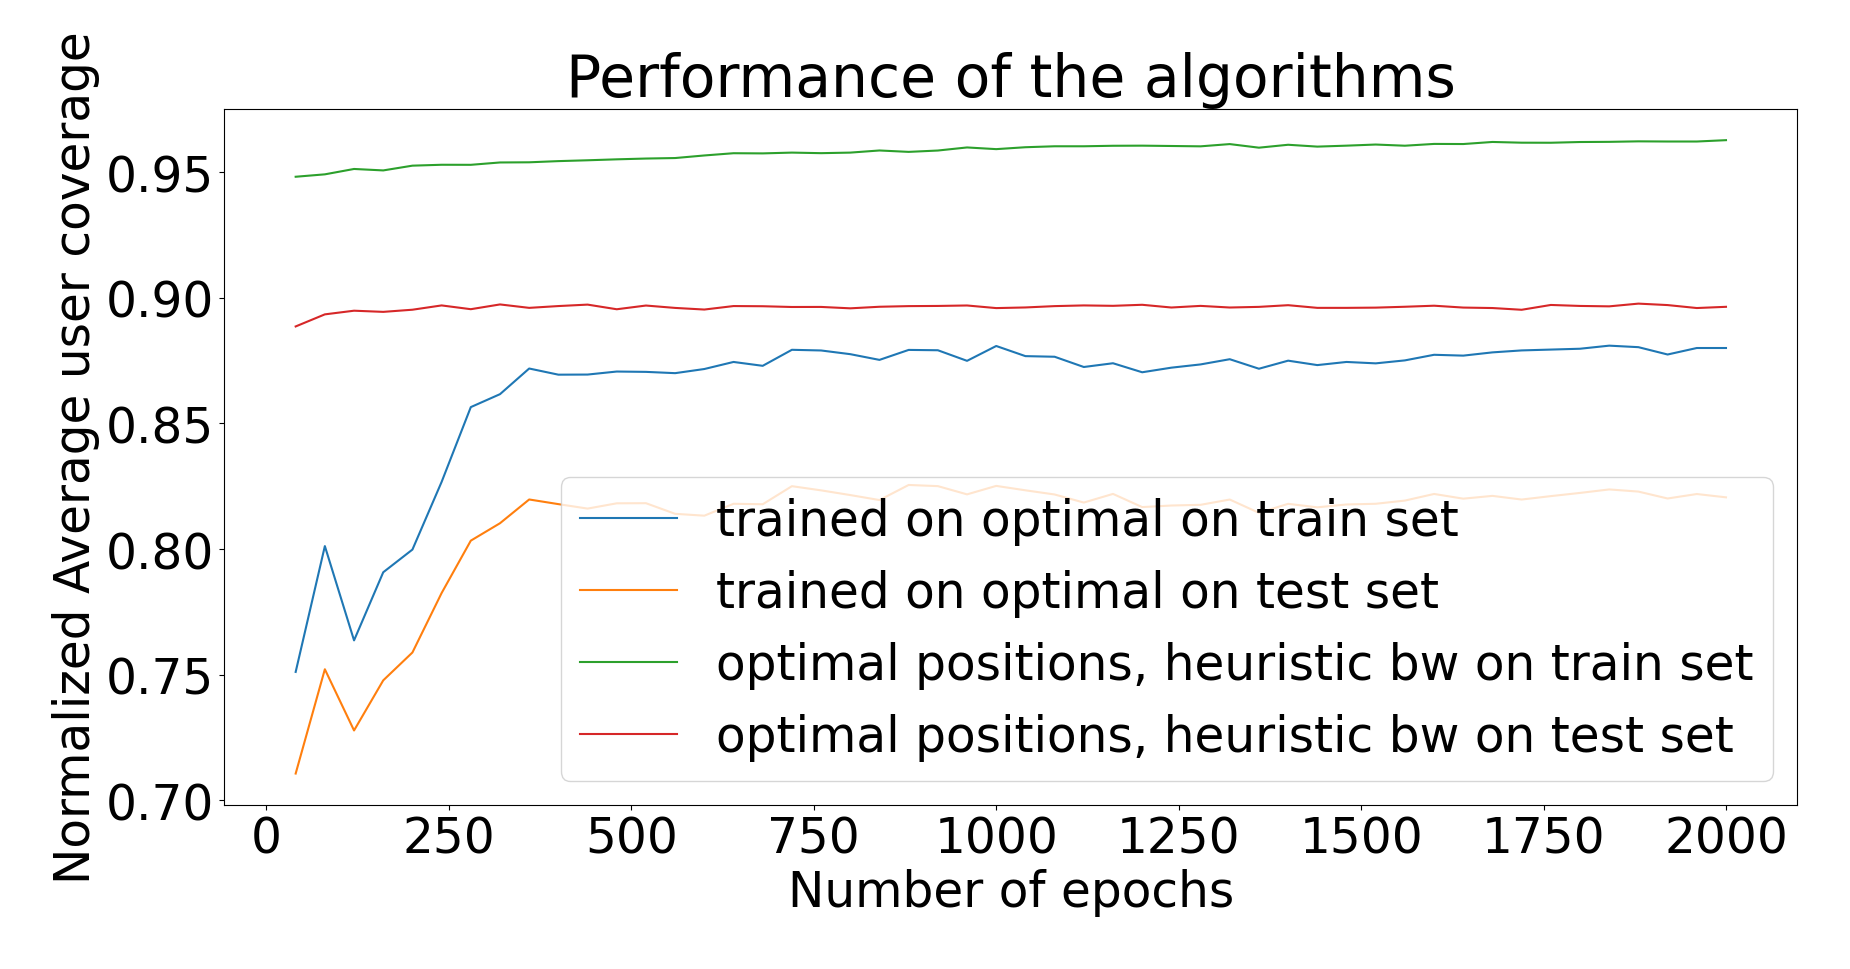
\includegraphics[width=0.5\textwidth]{images/bilan_en _fonction epochs_aibw.png}
    \caption{Performance with optimal positions and AI bandwiths}
\end{figure}

As we can see, the bandwidth part seems to be the issue, since even with perfect positions, the solution by the AI agent
is still far from perfect.

Thus, I implemented an agent which decides positions with a neural network, but decides the bandwiths optimally,
which is pretty fast once the positions are fixed.

We then have the following results:

\begin{figure}[H]
    \centering
    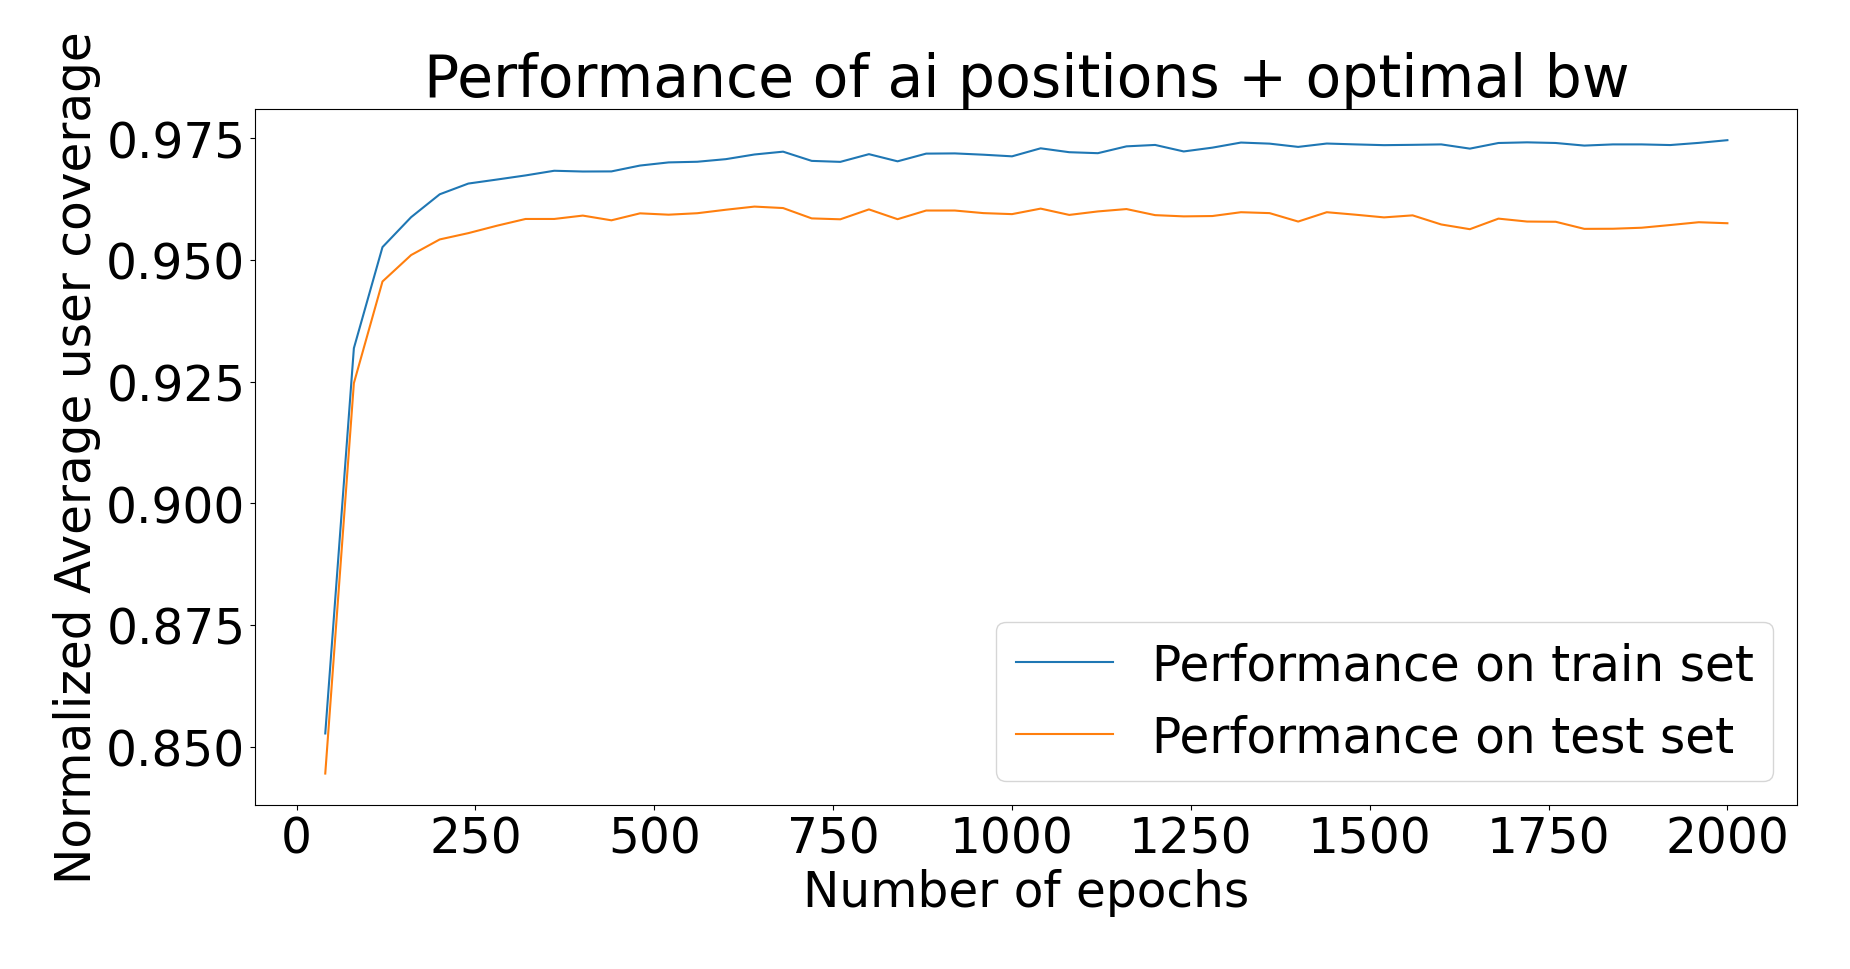
\includegraphics[width=0.5\textwidth]{images/mix_results.png}
    \caption{Performance with AI positions and optimal bandwiths}
\end{figure}

The results here are pretty convincing, but I will do a deep and honest analysis of the different methods in terms
of average reward but also in terms of average computation time.

\subsection{Generalizing to a variable number of users}

However, until now, I have only resolved instances with a fix number of users (50).

To fix this, the first solution we imagined was to use graph neural networks.
Graph neural networks (or gnn for short) are neural networks that are composed of a variable (i.e.\, not fixed) number
of nodes and edges and run some aggregated functions (like mean, min or max for example) on them to have a final answer.

The graph given to the neural network was constructed using a k-neighbourg algorithm.
I have made a graphic plotting the final test error on positions in function of the k in the k-neighbourg algorithm.

\begin{figure}[H]
    \centering
    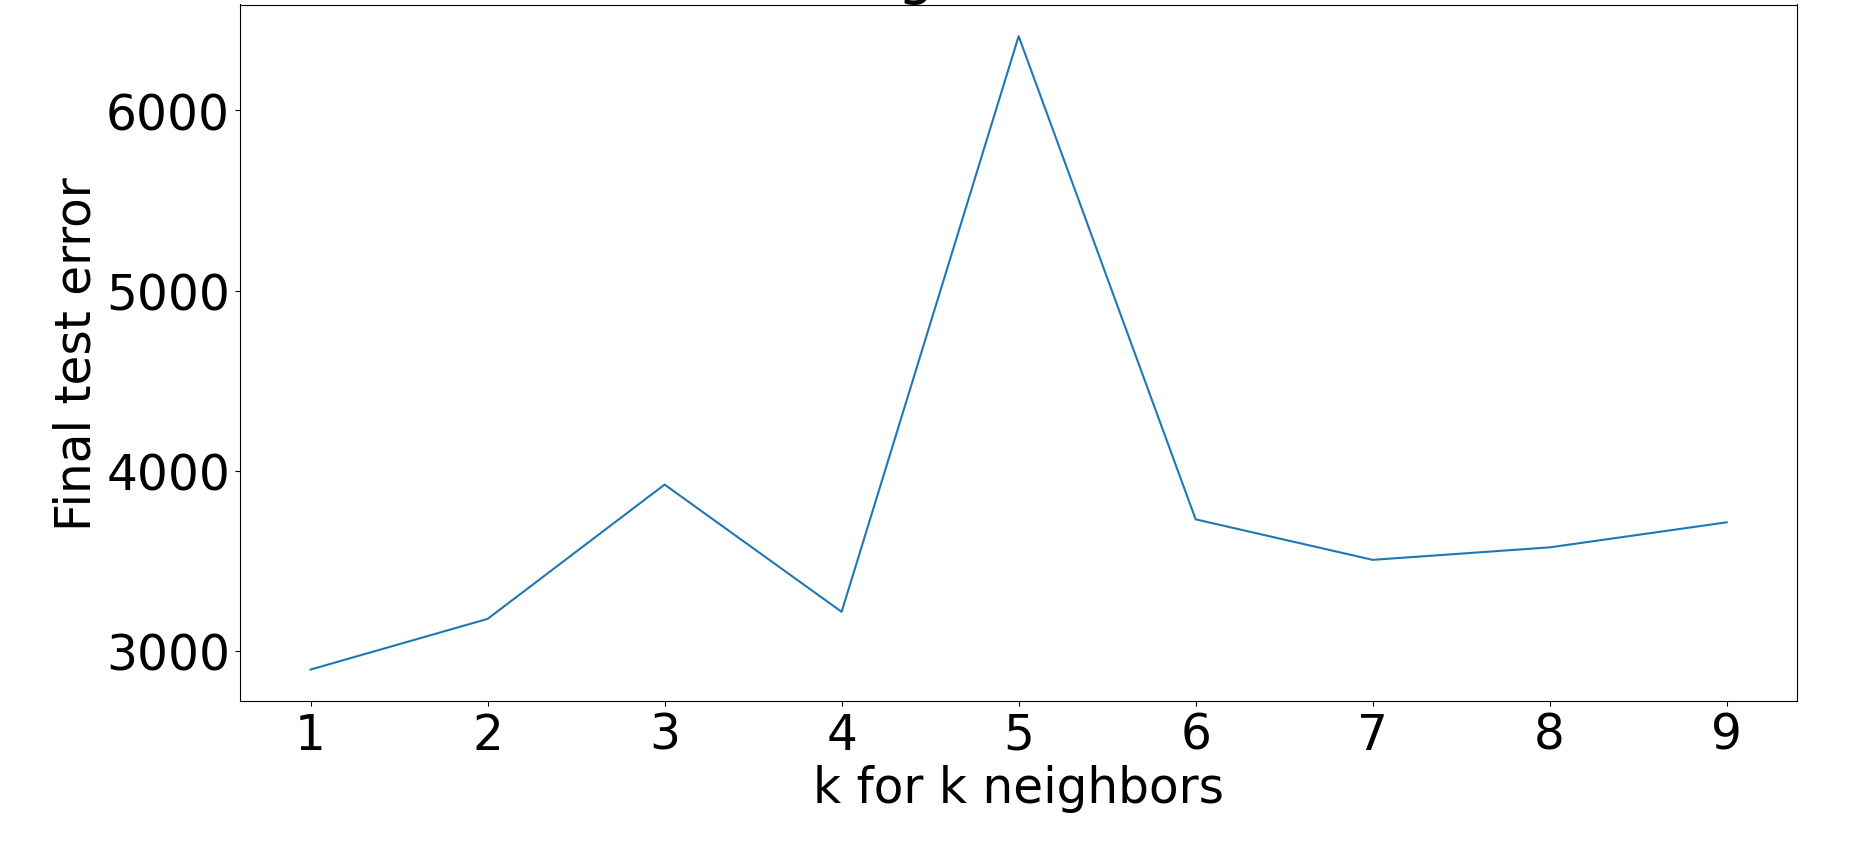
\includegraphics[width=0.5\textwidth]{images/knn_for_gnn.png}
    \caption{Position error for graph neural network in function of k}
\end{figure}

However, as you can see, whatever the chosen k is, the results are always lacking compared to what we had before.

I thus opted for a simpler but less scalable approach: I just add a one-hot to each user stating if the user exists or not.
Thus, the neural network can be used to resolve instances with a variable number of users, as long as the number in question is inferior to a certain maximum.

The precision on a variable number of users from 25 to 100 is very similar to what it used to be with a fix number of users as you can see in the following graphics:

\begin{figure}[H]
    \centering
    \begin{minipage}[b]{0.45\textwidth}
        \centering
        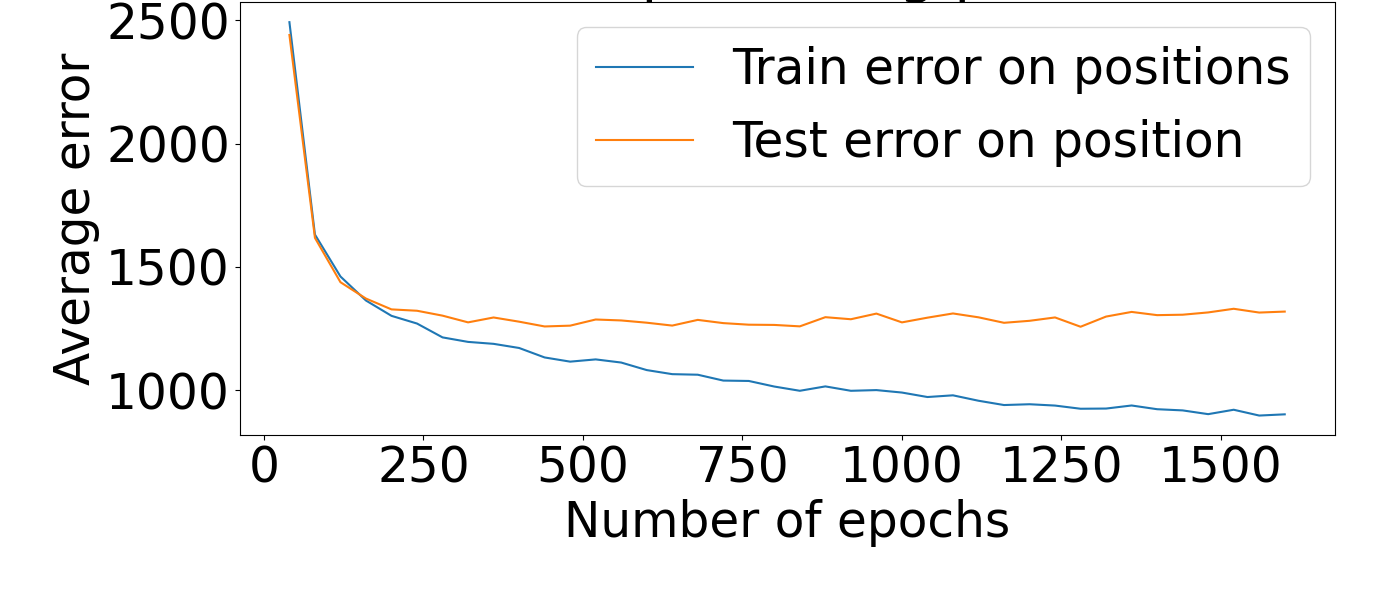
\includegraphics[width=\textwidth]{images/error_pos_variable_user_number.png}
        \caption{Position error}
    \end{minipage}
    \hspace{0.05\textwidth}
    \begin{minipage}[b]{0.45\textwidth}
        \centering
        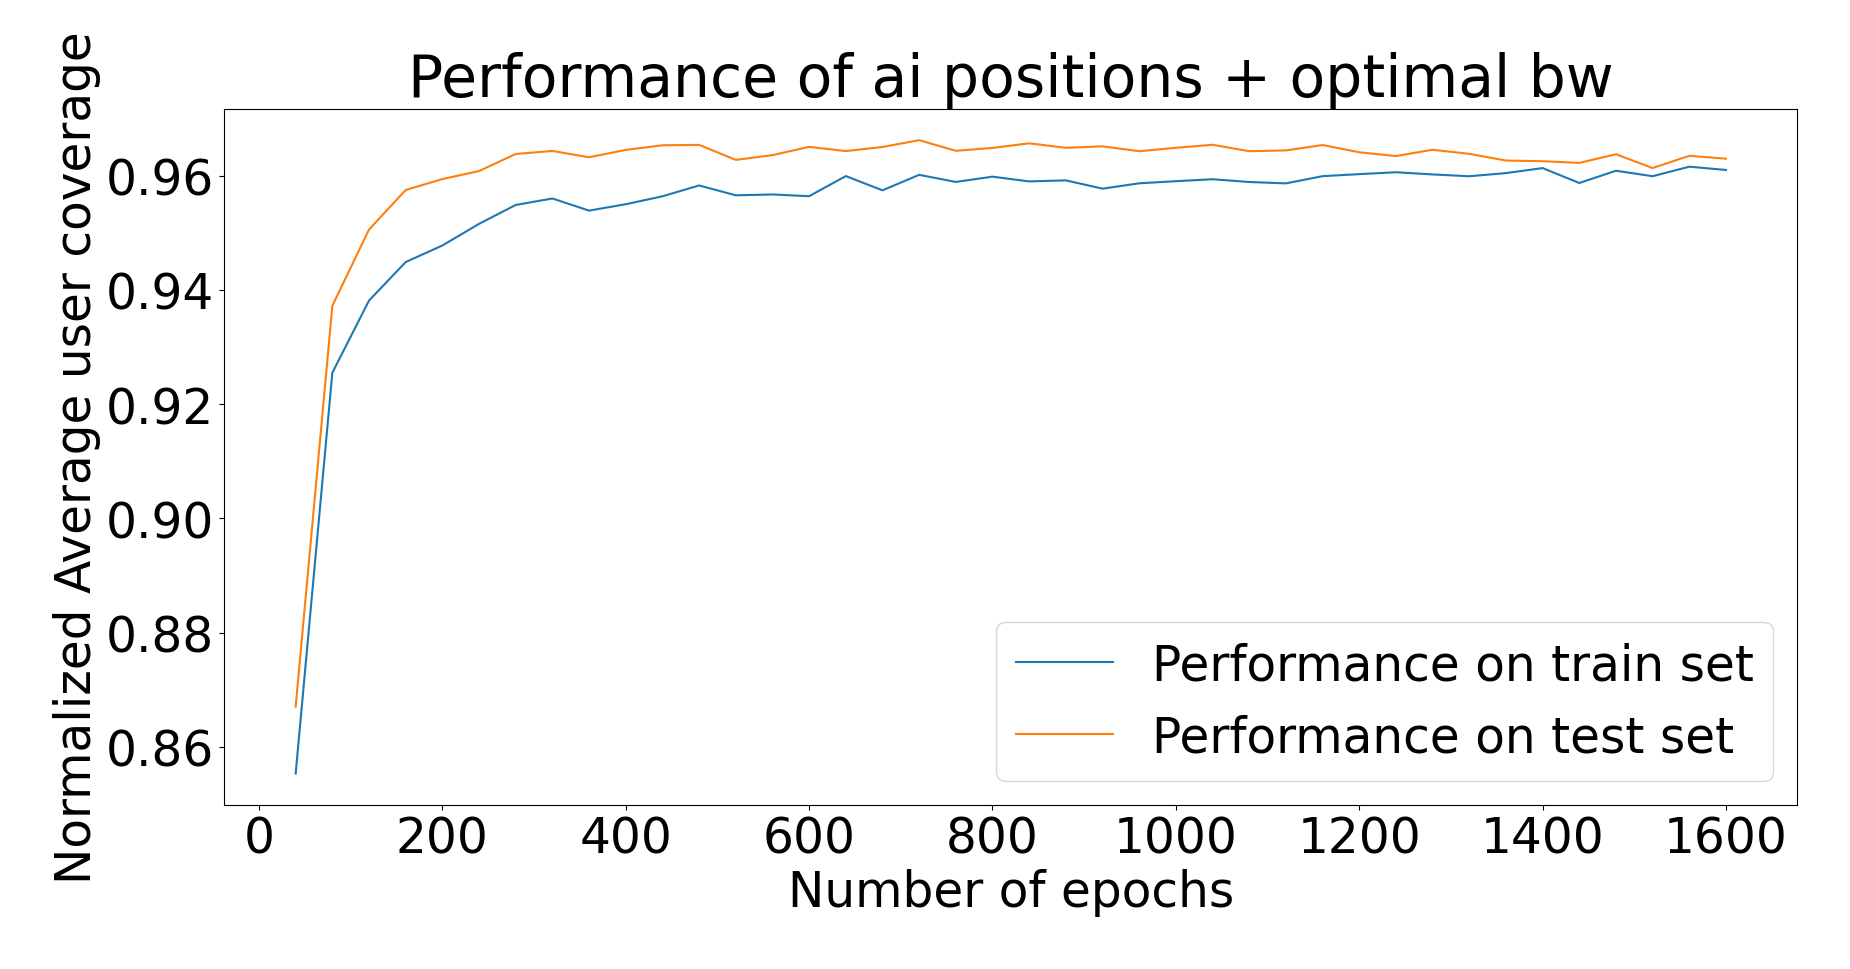
\includegraphics[width=\textwidth]{images/reward_variable_user_number.png}
        \caption{Average normalized reward}
    \end{minipage}
\end{figure}

\subsection{Comparaison of the different methods}

In this subsection I am going to compare the 3 agents we have seen in this article: the optimal agent, the full-ai agent and the hybrid agent.
The 2 criteria will be first average reward and second time computation.
Moreover, until now, I have always generated users in 2 clusters, which is the simplest case (and the one used in the article my internship is based on \,\cite{main_article}).
However, I will now evaluate the different agents on a number of clusters of 0 (which means random) to 4.

Let's start by evaluating the average reward.

\begin{center}
    \begin{tabular}{ c c c }
     Type of agent & random & 1 cluster \\ 
     Optimal & 50.25\% & 57.80\% \\  
     Full-ai & 32.81\% & 46.41\%  \\
     Hybrid &  36.82\% & 55.87\% 
    \end{tabular}
\end{center}


\section{Ouverture: Utiliser la distance à l'optimum comme erreur pour l'apprentissage}

\section{Conclusion}


\bibliographystyle{plain}
\bibliography{bibliography}


\appendix

\section{Appendix detailling how the neural networks are built}

For the position agent, each user is represented as:
\begin{enumerate}
    \item Its x and y axis
    \item A one-hot for each of the possible type
    \item A one-hot that indicates if the user actually exists (if the user does not exist, the positions are set to random and the one-hots above to 0)
\end{enumerate}

The number of users is easily adjustable (I set it to 100 in the tests)
The neural network is then composed of 2 convolutional layers, followed by 2 linear layers.
The hyper-parameters are the following: learning rate of $5e^{-5}$ and weight decay of $1e^{-5}$.

\;

For the bandwidth agent, each user is represented as before but there is an entry added for the position of each of the UAV.
The neural network is then composed of a convolutional layer for the drones, a convolutional layer for the users,
then the 2 results are concatenated and passed to 2 linear layers.
The hyper-parameters are the following: learning rate pf $2e^{-4}$ and weight decay of $1e^{-6}$



\end{document}


